%% -*- mode: latex; fill-column: 80; comment-column: 50; -*-
\documentclass[11pt,english]{article}

\usepackage[utf8]{inputenc}

\usepackage{pdfpages}
\usepackage{babel}
\usepackage{hyperref}
\usepackage{enumerate}
\usepackage{listings}
\usepackage{float}
\usepackage[justification=centering]{caption}
\usepackage{subcaption}
\usepackage{multirow}
\usepackage{diagbox}
\usepackage{amsmath}
\usepackage{amssymb}

\renewcommand*\ttdefault{lmtt}
\renewcommand*\sfdefault{lmss}

\DeclareMathOperator*{\argmax}{argmax}

\begin{document}

\author{Hao Chi KIANG}
\title{Introduction to Machine Learning: Lab 3}
\maketitle

\section*{Assignment 1: LDA and Logistic Regression}
\section*{Solution 1.1}
\autoref{lenwid} shows the carapace length and rear width of
the provided Australian Crabs data set. It seems there is
possibility to classify the crabs into two groups: the group
which tends to have higher position and the one that tends to
have lower position. Linear discriminant is a reasonable choice
here, as the gap between the cluster seems to be forming a
straight line.

\begin{figure}[H]
  \centering
  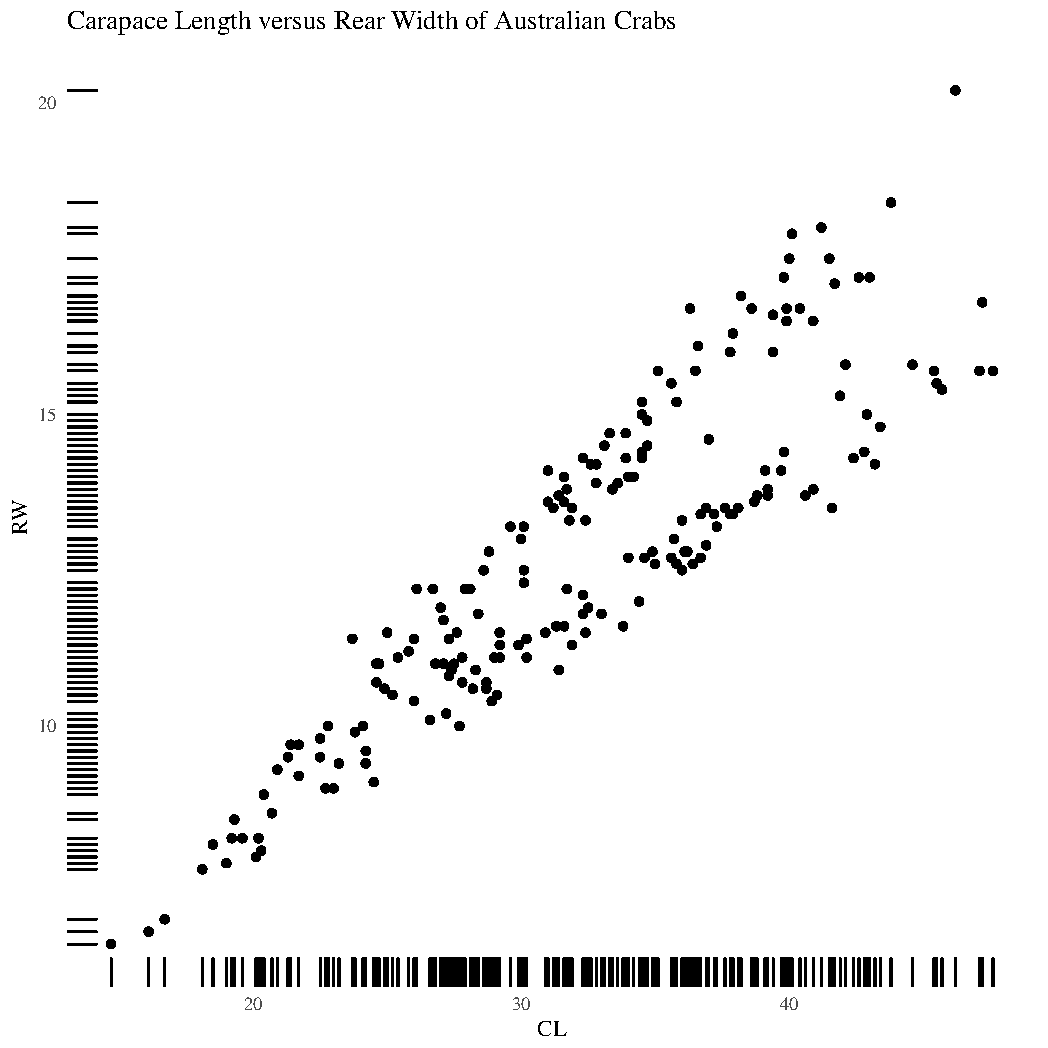
\includegraphics[width = 1.13\textwidth]{lenwid.pdf}
  \caption{Carapace Length versus Rear Width of Australian Crabs}
  \label{lenwid}
\end{figure}


\section*{Solution 1.2}
\autoref{lda} shows a classification result using linear discriminant
analysis, and a plot of the decision boundary is included.

\begin{figure}[H]
  \centering
  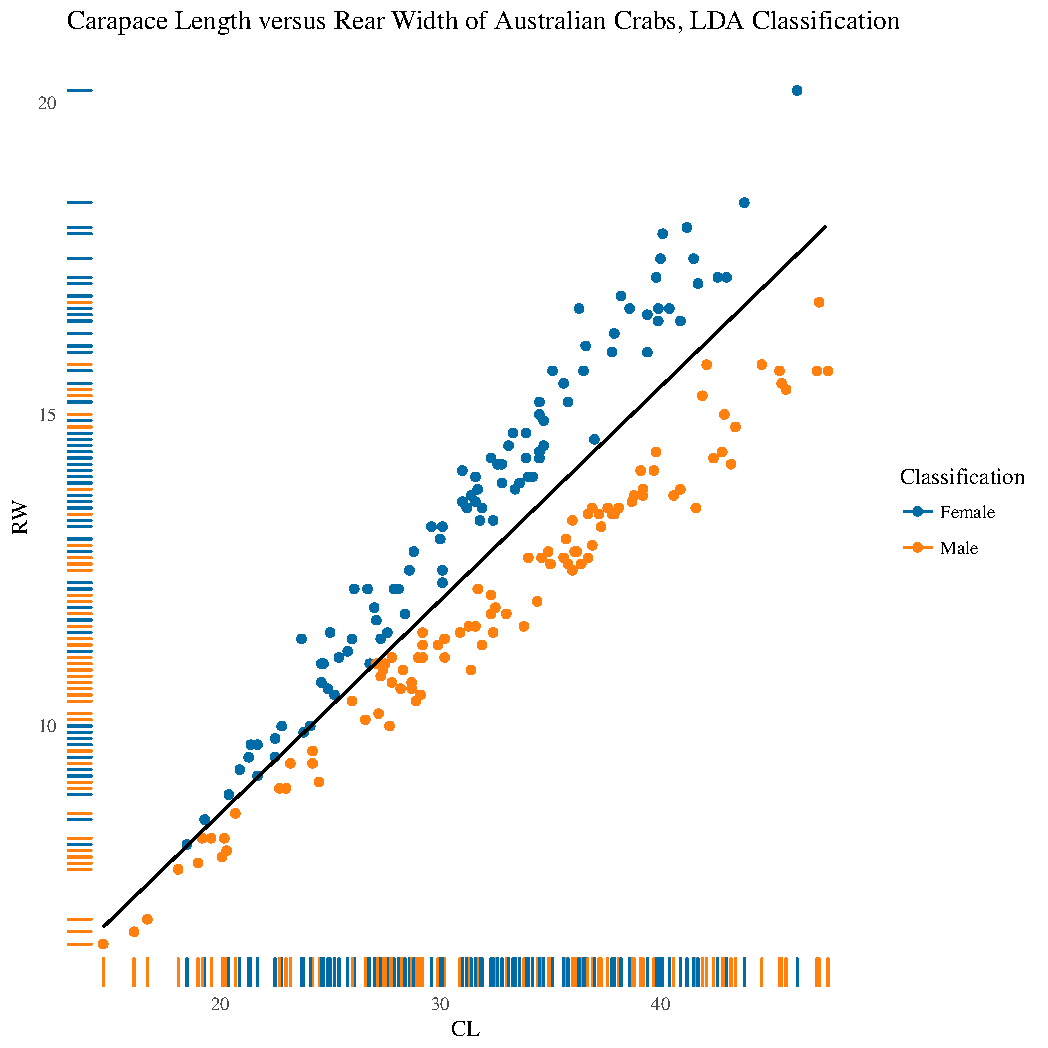
\includegraphics[width = 1.13\textwidth]{lda.pdf}
  \caption{Carapace Length versus Rear Width of Australian Crabs,
    Classification result}
  \label{lda}
\end{figure}

The estimated discriminant function is
\begin{align*}
  \delta_i(x_1, x_2) = w_{0i} + w_{1i}x_1 + w_{2i}x_2
\end{align*}
where $i$ is the identification number of features: CL be 1, and RW be 2,
and $w_{ij}$ have the following estimated values:
\begin{align*}
&w_{01} = -12.6833192,&\quad& w_{02} = -22.648321 \\
&w_{11} = -0.2159742,&\quad& w_{12} = -2.183150 \\
&w_{21} = 2.5917691,&\quad& w_{22} = 8.332018
\end{align*}

The equation of decision boundary can be derived easily as follow:
The set of points $(x_1, x_2)$ on the boundary are the points which
satisfies $\delta_1(x_1, x_2) = \delta_2(x_1, x_2)$. That is,
\begin{align*}
  w_{01} + w_{11}x_1 + w_{21}x_2 = w_{02} + w_{12}x_1 + w_{22}x_2
\end{align*}

Plugging in our value of estimated $w_{ij}$ and normalize on $x_1$'s term,
term, the equation is
\begin{align*}
  x_1 - 2.918x_2 + 5.066 = 0
\end{align*}

This function was used to plot the boundary with $ggplot$.

\section*{Solution 1.3}
\autoref{realdat_lda} displays the decision boundary and the real data on
the same plot. We can see that our classification is quite accurate.

\begin{figure}[H]
  \centering
  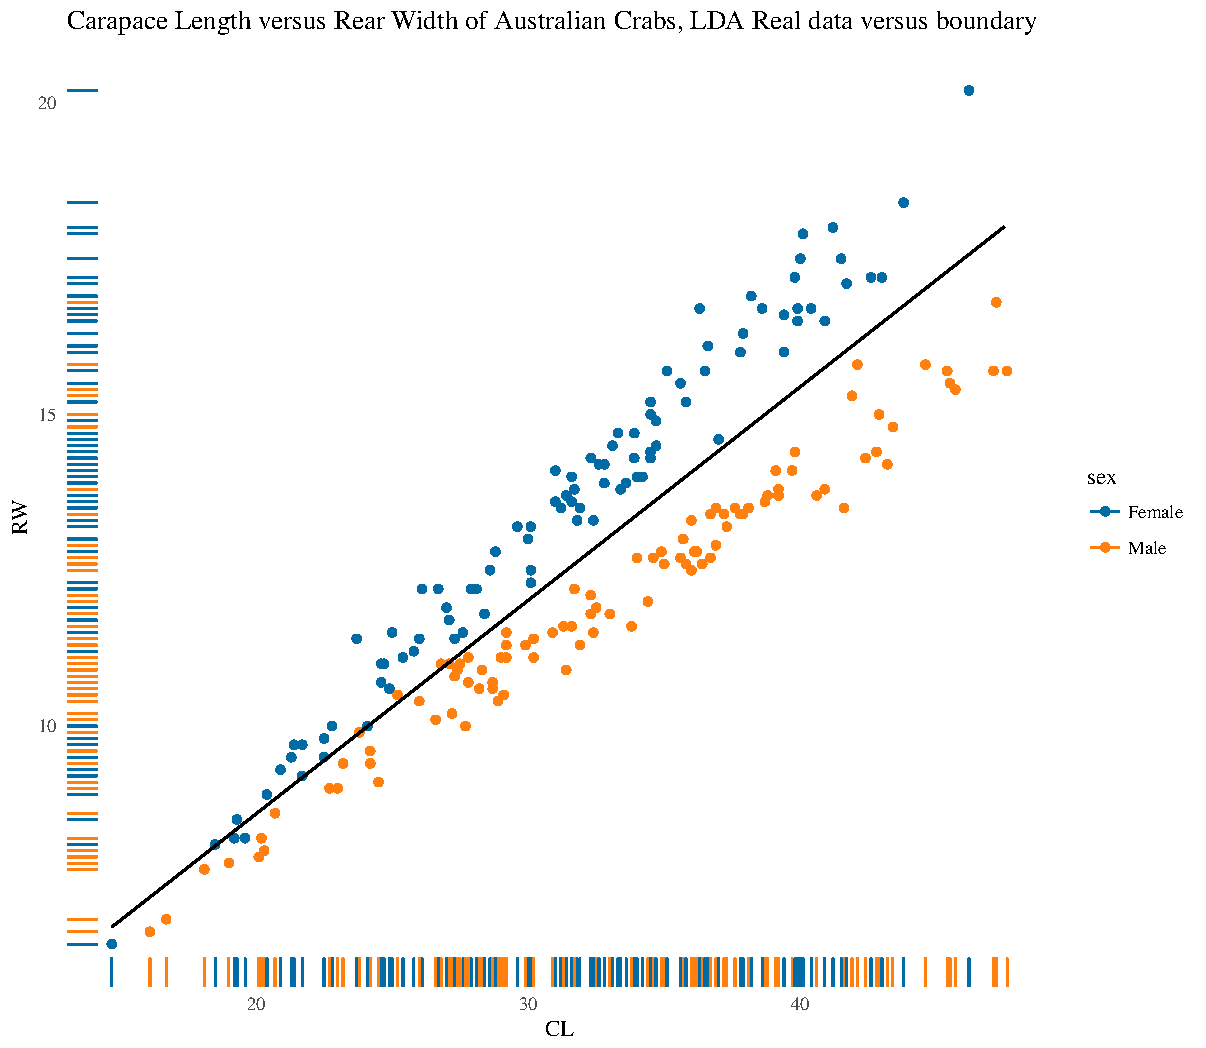
\includegraphics[width = 1.13\textwidth]{realdat_lda.pdf}
  \caption{Carapace Length versus Rear Width of Australian Crabs, Real data
  vs. Decision Boundary}
  \label{realdat_lda}
\end{figure}

\section*{Solution 1.4}

\autoref{glm} shown a logistic regression using the $glm()$ function. The
result of logistic regression is almost exactly the same as the 

\begin{figure}[H]
  \centering
  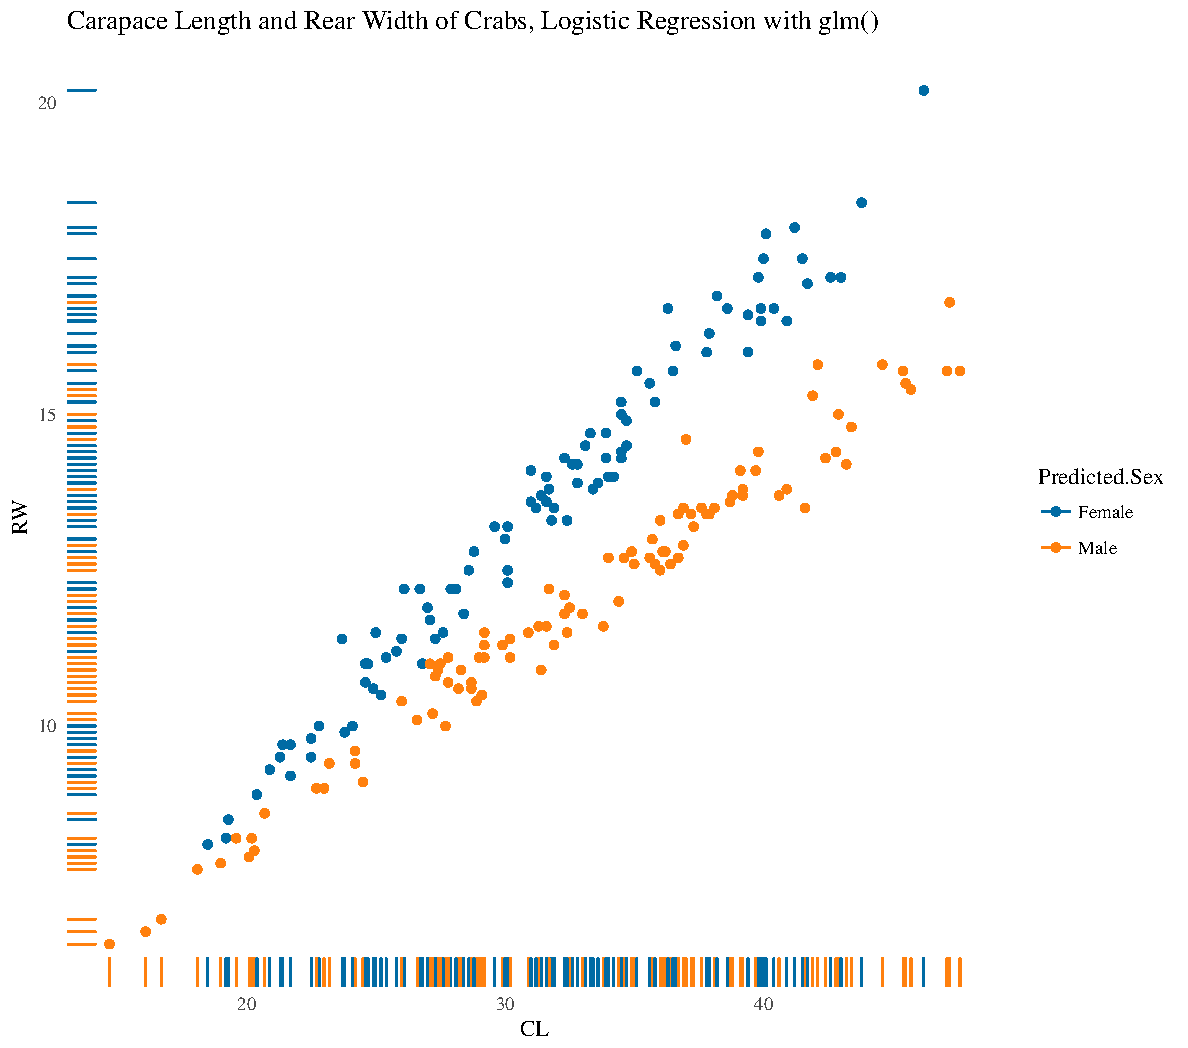
\includegraphics[width = 1.13\textwidth]{glm.pdf}
  \caption{Carapace Length and Rear Width of
    Crabs, Logistic Regression with glm()}
  \label{glm}
\end{figure}

The equation of decision boundary can be derived as follows:

Consider any general logistic function $f(x) = \frac{1}{1+e^{-x}}$.
The solution of the equation $f(x) = 1 - f(x)$ is
\begin{align*}
  \frac{1}{1+e^{-x}} &= 1 - \frac{1}{1+e^{-x}}\\
  \frac{1}{1+e^{-x}} &= \frac{e^{-x}}{1+e^{-x}}\\
  1 &= e^{-x}\\
  x &= 0
\end{align*}\label{logproof}
Now we want to find the set of points $(x_1, x_2)$ whose probabilty
of being female is the same as being male. That is, we want a set of points
which satisfy $f(w_0 + w_1x_1 + w_2x_2) = 1 - f(w_0 + w_1x_1 + w_2x_2)$, where
$w_i$ are the linear regression coefficients. By \ref{logproof}, this set of
points satisfies
\begin{equation}
  w_0 + w_1x_1 + w_2x_2 = 0
\end{equation}
Plugging in our estimated $w_i$ and normalize on $x_1$'s term, the
equation is
\begin{equation}
  x_1 - 2.713x_2 + 2.940 = 0
\end{equation}
This is very similar to to the result we got from logistic regression.


\section*{Assignment 2: Linear Regression and Regularization}


\subsection*{Solution 2.1, 2.2}
The misclassification rate is as below:\\

\begin{tabular}{ l l }
  Gini Train & 0.236 \\
  Gini Testing & 0.36 \\
  Deviance Train & 0.212 \\
  Deviance Testing & 0.268
\end{tabular}
\\\\\\
From the above table, deviance seems to be a better measure of impurity in our
data set.

\subsection*{Solution 2.3}
According to \autoref{treedepth}, it is reasonable to use tree depth = 4
as the best tree for prediction. The tree uses savings, duration, and
history as predictor, which is very consistent to our common sense.
The misclassification rate for testing data of this tree is $0.256$.

\begin{figure}[H]
  \centering
  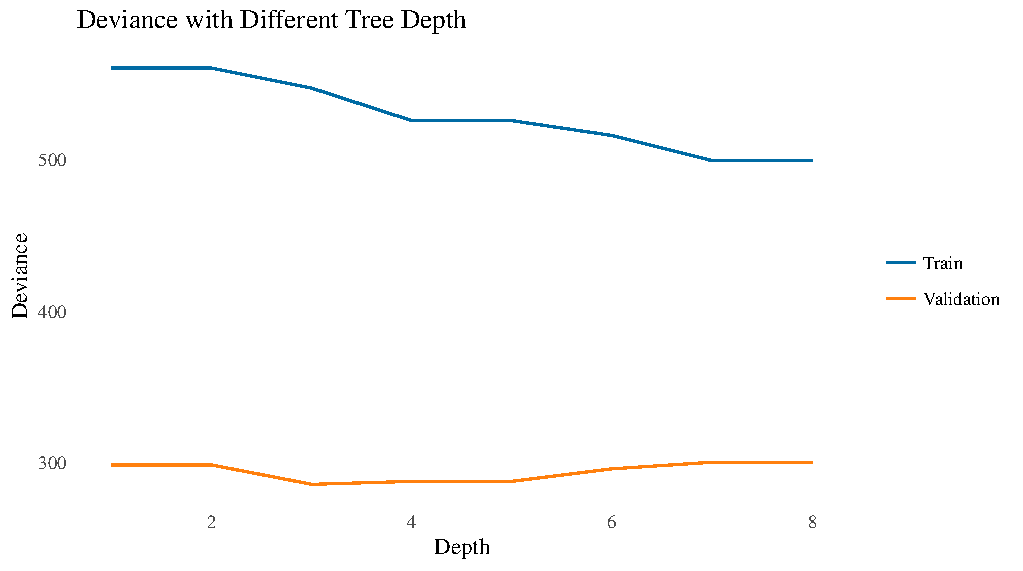
\includegraphics[width = 1.13\textwidth]{treedepth.pdf}
  \caption{Deviance with Different Tree Depth}
  \label{treedepth}
\end{figure}


\subsection*{Solution 2.4}
The confusion matrix of Naive Bayes classification using the training data set
is as follows:\\\\
\begin{tabular}{ l | l | l }
  & bad & good \\
  \hline
  bad & 95 & 98 \\
  good & 52 & 255
\end{tabular}
\\\\\\
Misclassification rate of training data is $0.3$.
The confusion matrix using the testing data set is as follows:\\\\
\begin{tabular}{ l | l | l }
  & bad & good \\
  \hline
  bad & 46 & 49 \\
  good & 30 & 125
\end{tabular}
\\\\\\
Misclassification rate of testing data is $0.316$. The classification is
significantly worse than that of decision tree.

\subsection*{Solution 2.5}
The confusion matrix of Naive Bayes classification with the provided
custom loss function and the training data set is as follows:\\\\
\begin{tabular}{ l | l | l }
  & bad & good \\
  \hline
  bad & 27 & 17 \\
  good & 120 & 336
\end{tabular}
\\\\\\
Misclassification rate of training data is $0.274$.
The confusion matrix using the testing data set is as follows:\\\\
\begin{tabular}{ l | l | l }
  & bad & good \\
  \hline
  bad & 14 & 10 \\
  good & 62 & 164
\end{tabular}
\\\\\\
Misclassification rate of testing data is $0.288$. This classification
gives better overall misclassification rate, but it is more likely
misclassify bad loaners as good: it is very conservative. The fact that
such a conservative criterion gives better overall rate than that using
normal loss function is due to that the normal loss function is more
likely misclassify good loaner as bad: the adjustment of loss function
corrected these bias. Also, most of the customers are good anyway, so
adjusting the algorithm to guess more 'good' doesn't harm much.

\newpage
\lstset{
  frame=single,
  basicstyle=\ttfamily\footnotesize,
  commentstyle=\color{gray},
  frame=L,
  language=R,
  showstringspaces=false,
}

\section*{Appendix 1: R Codes}
\label{ax1}
\lstinputlisting{worksheet1.R}


\end{document}

